\chapter{Related Protocols}
\label{chapter:first-appendix}

\section{JSON}

JavaScript Object Notation (JSON) is a text format for the serialisation of structured data. It is derived from the object literals of JavaScript, as defined in the ECMAScript Programming Language Standard \cite{crockford2006application}. JSON has numbers, strings, booleans and null as its primitive types. Additionally, it has objects and arrays as structured types. JSON becomes popular to exchange data between in web services or applications. With JSON, WAMP message payload is serialisable and provides data types according to those of JSON. 

\section{URI}

Uniform Resource Identifiers (URIs) provide a simple and extensible means for identifying a resource. URIs have a global scope and are interpreted consistently regardless of context \cite{masinter2005uniform}. WAMP binds to URIs by default, then it assumes global assignments and resolution to be unique. URIs are used as IDs for both topics in Pub/Sub and procedures in RPC. 

\section{XML}
Extensible Markup Language (XML) is a markup language that was designed to transport and store data. Furthermore, XML was designed to be self-describing and can be used straightforward over the Internet. XML has been widely used, for example, the SOAP protocol that we mentioned in the thesis. 


\chapter{Screenshots}
\label{chapter:second-appendix}

\section{Web-based IoT Applications Screenshots}

\subsection{Smart Lighting and Control Application}

Figure \ref{fig:screen-shot-home-auto} shows the visualisation of the lights changing according to the sun brightness, for the purpose of keeping the light brightness in a constant level.

\begin{figure}[ht]
  \begin{center}
    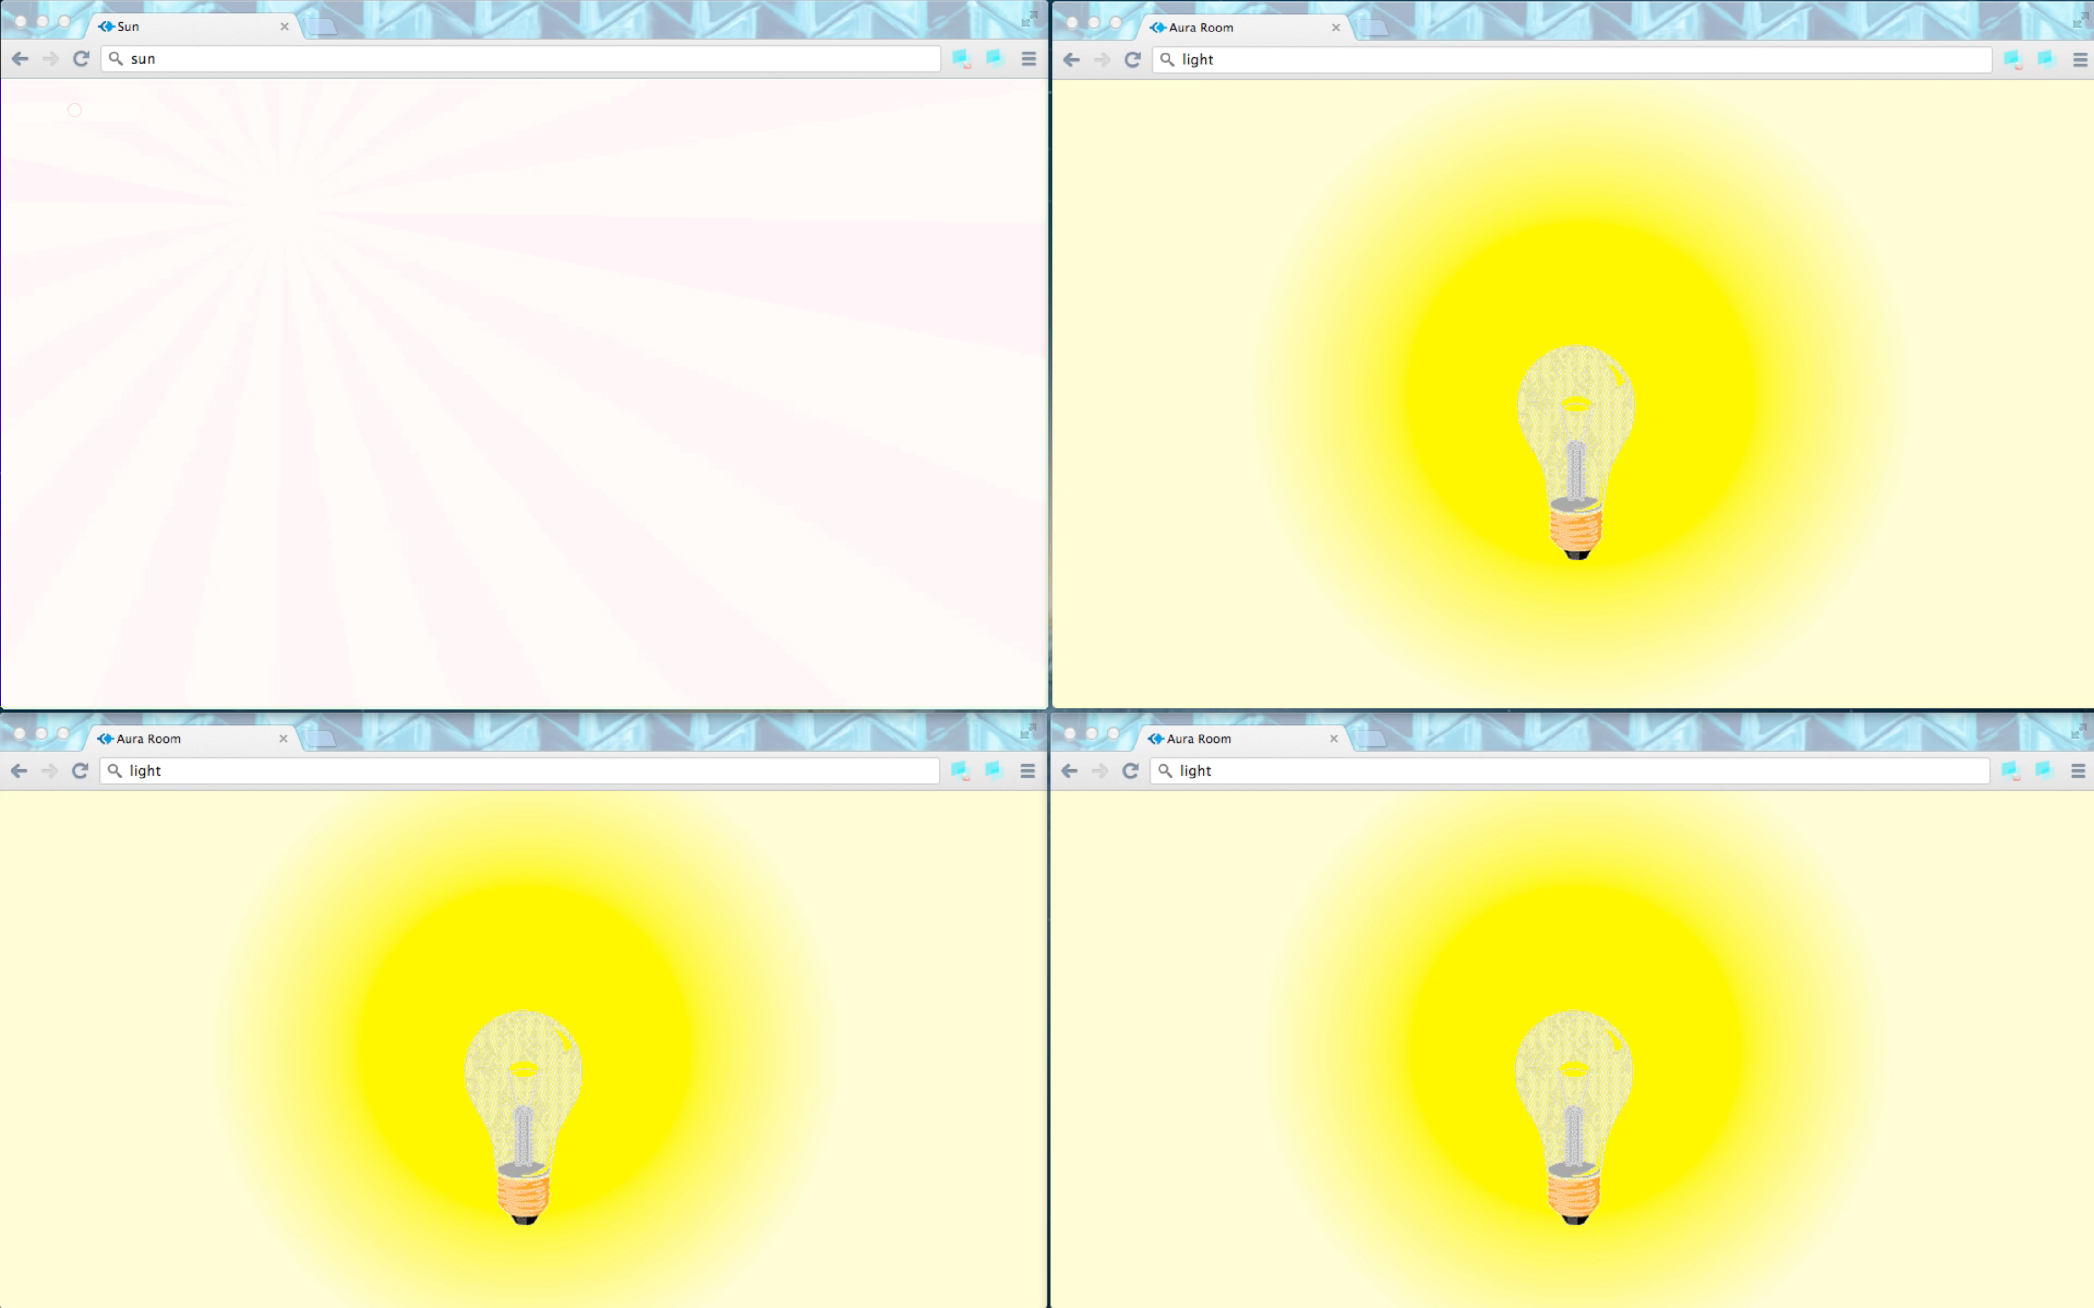
\includegraphics[width=1\textwidth]{images/screen-shot-home-auto.pdf}
    \caption{Visualisation of Lights Changing According to the Sun}
    \label{fig:screen-shot-home-auto}
  \end{center}
\end{figure}

Figure \ref{fig:screen-shot-home-auto-2} shows the visualisation of remote controlling lights status.

\begin{figure}[ht]
  \begin{center}
    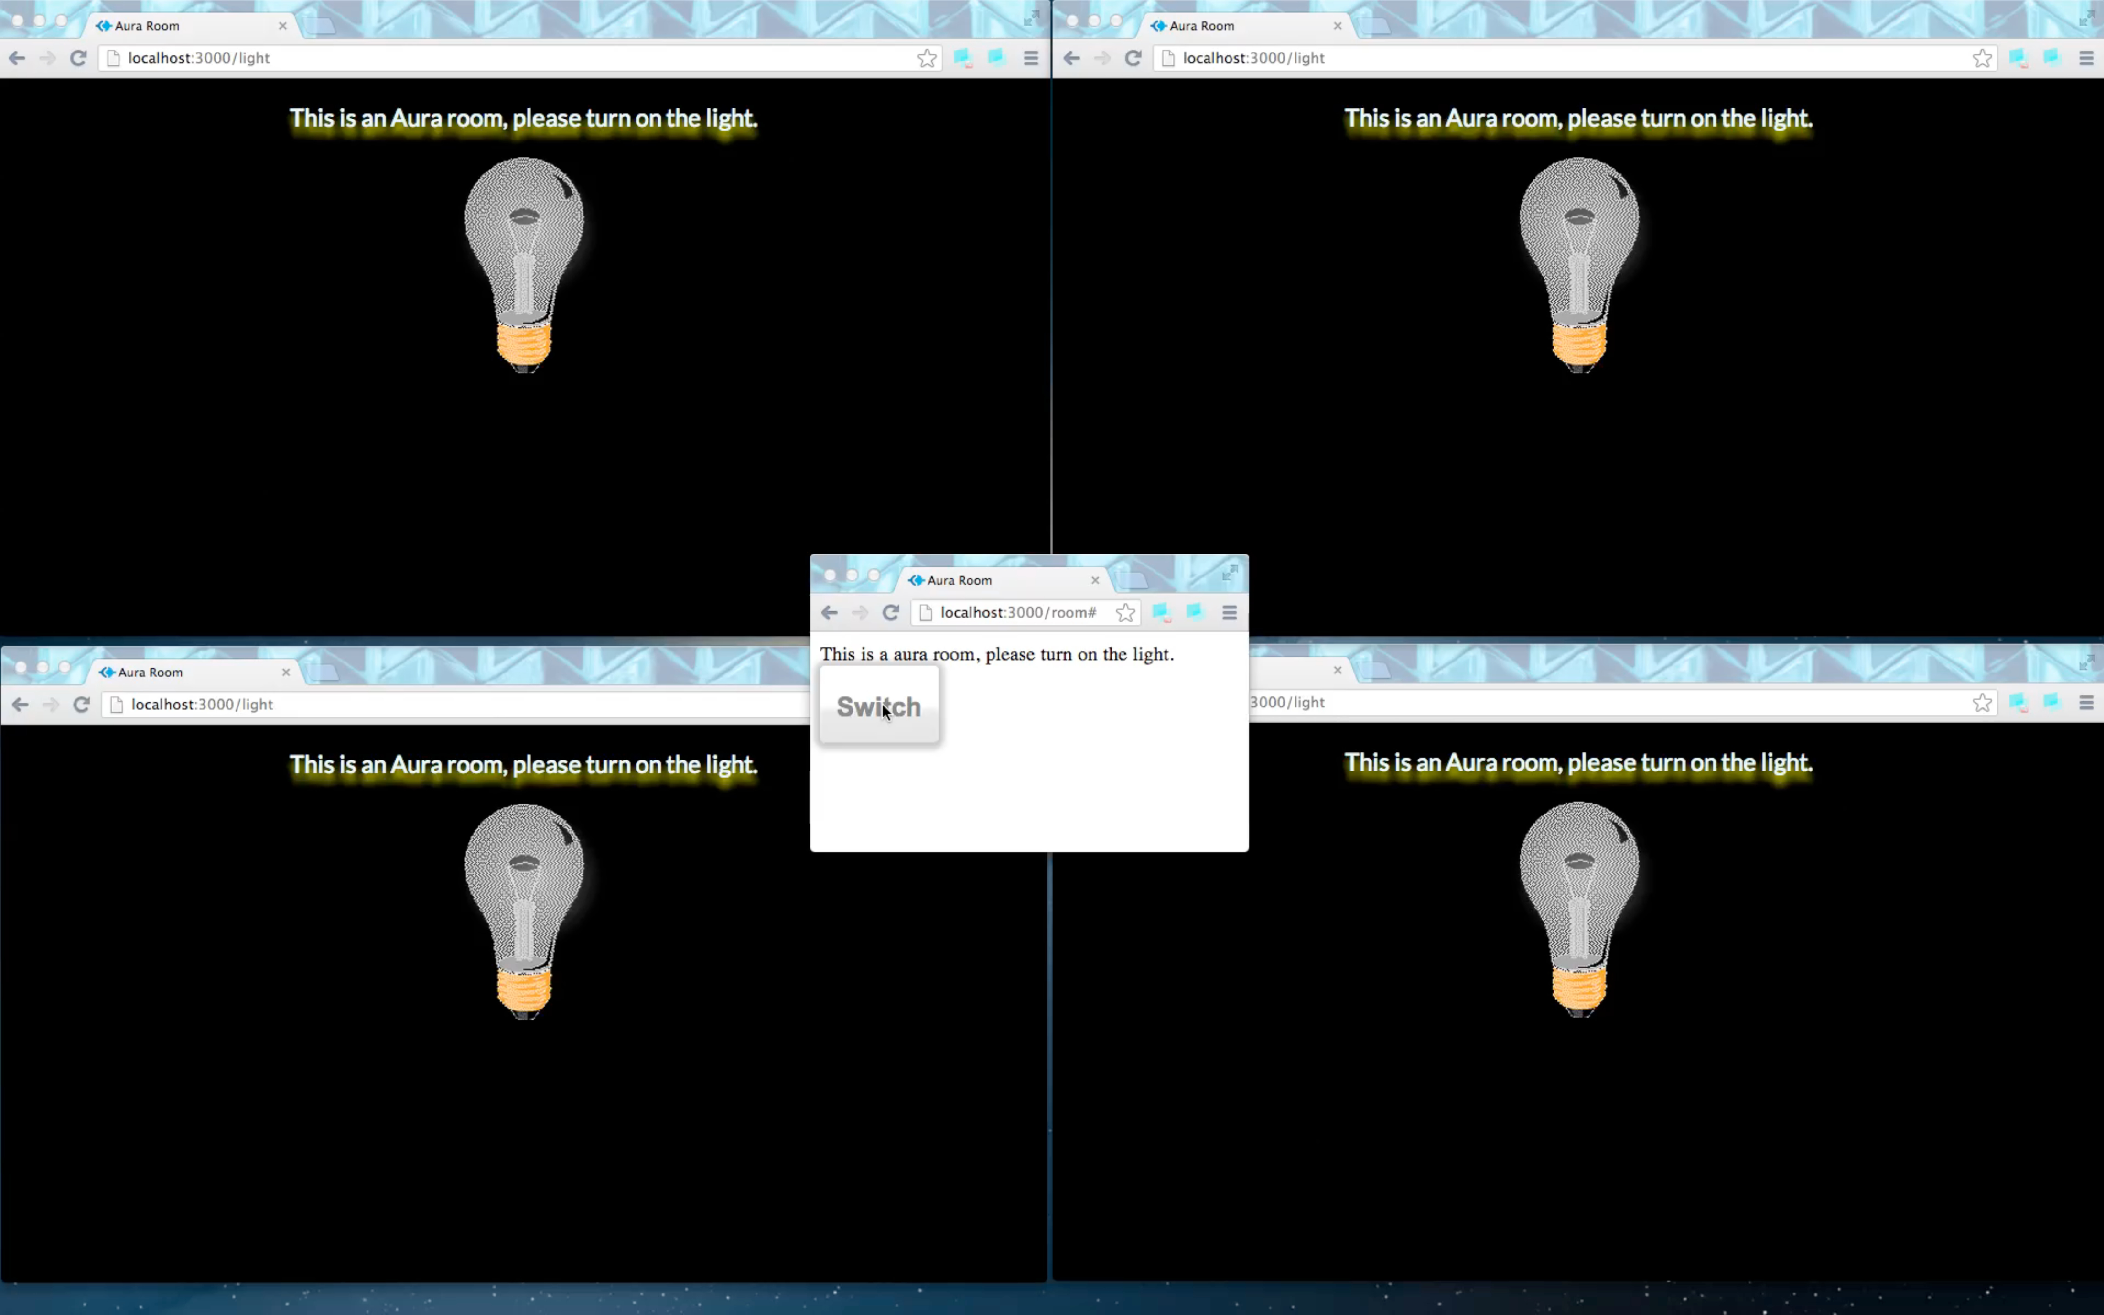
\includegraphics[width=1\textwidth]{images/screen-shot-home-auto-2.pdf}
    \caption{Visualisation of Remote Controlling Lights}
    \label{fig:screen-shot-home-auto-2}
  \end{center}
\end{figure}

\subsection{Social Sensing Application}

Figure \ref{fig:screen-shot-social-sensing-map} shows the social sensing application based on geo-location. The density of the nodes is visualised in heat map. This is, the colour scale is the reflection of the number of nodes at a place.

\begin{figure}[ht]
  \begin{center}
    \includegraphics[width=1\textwidth]{images/screen-shot-social-sensing-map.pdf}
    \caption{Visualisation of Social Sensing based on Geo-location}
    \label{fig:screen-shot-social-sensing-map}
  \end{center}
\end{figure}

Figure \ref{fig:screen-shot-social-sensing-netowrk} shows the social sensing application based on nodes interconnection.

\begin{figure}[ht]
  \begin{center}
    \includegraphics[width=1\textwidth]{images/screen-shot-social-sensing-netowrk.pdf}
    \caption{Visualisation of Social Sensing based on Nodes Interconnection}
    \label{fig:screen-shot-social-sensing-netowrk}
  \end{center}
\end{figure}
Figure \ref{fig:screen-shot-social-sensing-network-data} shows the visualisation of data in database-centric approach.

\begin{figure}[ht]
  \begin{center}
    \includegraphics[width=1\textwidth]{images/screen-shot-social-sensing-network-data.pdf}
    \caption{Visualisation of Data in Database-centric Approach}
    \label{fig:screen-shot-social-sensing-network-data}
  \end{center}
\end{figure}